\chapter{Multiscale turbulence measurements}
\label{ch:TurbulenceMeasurements}
Development of a first-principles understanding
of turbulent transport in a tokamak
requires multi-tiered validation\ldots
comparing not just heat fluxes, but
also turbulent spectra etc.
\diiid's extensive suite of fluctuation diagnostics
provides an ideal setting to validate
predicted changes~\cite{howard_pp16}
to turbulent spectra when altering relative drive
between electron-scale and ion-scale turbulence.


\section{Overview of multiscale gyrokinetic predictions}


\section{Experimental conditions}
The experiment was run in the ITER-similar shape,
with aspect ratio, elongation, and triangularity
all closely matched to those of the ITER-baseline scenario
\cite[Sec.~13.5 \& 13.6]{wesson}.
The on-axis toroidal field $B_T = \SI{1.7}{\tesla}$ and
plasma current $I_p = \SI{1.3}{\mega\ampere}$
produced $q_{95} = 3.15$,
where $q_{95}$ is the average value
of the safety factor $q$~\cite[Sec.~3.4]{wesson}
over the surface that encloses $95\%$
of the poloidal flux within the last-closed flux surface.
Neutral beam injection (NBI)~\cite[Sec.~5.3-5.5]{wesson}
was performed with feedback to maintain
$\beta_N = 1.9$, where
$\beta_N$ is the normalized plasma pressure~\cite[Sec.~6.18]{wesson}.
In order to suppress core MHD,
an average NBI torque of approximately $\SI{1.5}{\newton \meter}$
was injected into the plasma;
note that this is approximately four times larger than
the projected ITER-equivalent torque~\cite{garofalo_nf11}.
In order to alter the local electron-scale and ion-scale drives,
the electron cyclotron resonance heating (ECH)~\cite[Sec.~5.10]{wesson}
location was scanned between $\rho = 0.5$ and $\rho = 0.8$,
where $\rho$ is the square root of the normalized toroidal flux
(which scales as $r / a$, with
$r$ being the minor-radial coordinate and
$a$ being the minor radius of the plasma).
Intra-shot scans of the ECH location
were plagued with core MHD, so
only shot-to-shot, MHD-free scans of the ECH location
are considered here.
The line-averaged density was
$\bar{n}_e = \SI{5.2e19}{\per\meter\cubed}$.
Impurities were removed from the plasma
by both large and small edge localized modes (ELMs)~\cite[Sec.~7.17]{wesson}.
The time histories of several actuators and plasma parameters
are shown in Figure~\ref{fig:TurbulenceMeasurements:traces}.
Note that multiscale gyrokinetic simulations
of this experiment's reference discharge,
\diiid\space shot $153523$ with ECH at $\rho = 0.5$,
indicate that the turbulent transport
is intrinsically multiscale in nature~\cite{holland_nf17}.

\begin{figure}
  \centering
  \includegraphics[width = \textwidth]{%
    Chapters/TurbulenceMeasurements/figs/traces.png}
  \caption[Time histories of various actuators \& plasma parameters]{%
    Time histories of various actuators and plasma parameters:
    (a) electron cyclotron resonance heating (ECH) power $P_{\text{ECH}}$,
    (b) ECH location $\rhoech$,
    (c) neutral beam injected (NBI) power $P_{\text{inj}}$,
    (d) NBI torque $T_{\text{inj}}$,
    (e) line-averaged density $\bar{n}_e$,
    (f) normalized plasma pressure $\beta_N$,
    (g) confinement quality $H_{98,\text{y}2}$, and
    (h) divertor $D_{\alpha}$ light, indicating
    the presence of large and small edge localized modes (ELMs).
  }
\label{fig:TurbulenceMeasurements:traces}
\end{figure}

Equilibrium profiles were obtained
by averaging over $\SI{200}{\milli\second}$,
as indicated by the shaded regions
in Figure~\ref{fig:TurbulenceMeasurements:traces}.
Magnetic equilibria were
reconstructed with the EFIT code~\cite{lao_fst05} and
were constrained to match the total plasma pressure and
motional Stark effect (MSE) measurements
of the local magnetic pitch angle.
Electron densities and temperatures
were measured via Thomson scattering, while
ion densities and temperatures
were inferred from charge exchange recombination (CER) measurements
of C$^{6+}$, the dominant impurity in \diiid.
The radial electric field was computed
by invoking force balance on C$^{6+}$.
% (poloidal data for $\rho \geq 0.6)$
To minimize the impact of ELMs on the profile fits,
only measurements falling
within the last {$50\%$ -- $99\%$} of each inter-ELM window
were included in the fitting.
The fitted profiles and
their corresponding gradients or
\textcolor{red}{normalized inverse scale lengths}
are shown in
Figure~\ref{fig:TurbulenceMeasurements:profiles}.
While it may seem counterintuitive
that the central electron temperature $T_e(0)$
increases when moving ECH from $\rho = 0.5$ to $\rho = 0.8$,
maintaining constant $\beta_N$
requires increased NBI heating
(see Figure~\ref{fig:TurbulenceMeasurements:traces}(c)),
which enhances the NBI electron heating density $q_{e,\text{NBI}}$
across the full plasma profile,
as shown in Figure~\ref{fig:TurbulenceMeasurements:electron_heating}(b).
The $1\sigma$ uncertainties in the profile fits,
indicated by the shaded bands in
Figure~\ref{fig:TurbulenceMeasurements:profiles},
were quantified by
performing separate fits to $100$ distinct data sets
generated via Monte Carlo variation
of the measurements about their uncertainties.
Clearly, moving ECH from $\rho = 0.5$ to $\rho = 0.8$
produces large changes
in the electron-scale and ion-scale drives,
$a / L_{T_e}$ and $a / L_{T_i}$, respectively,
in the region of the plasma accessible to the PCI probe beam
($R \geq \SI{1.98}{\meter}$).
Using these profiles,
power-balance analysis was performed
with the \textcolor{red}{ONETWO} code,
with NUBEAM~\cite{pankin_cpc04} calculations
for NBI heating and torque and
TORAY~\cite{matsuda_ieee89} calculations for ECH;
the resulting loop voltages, stored energies, and neutron rates
match their measured values to within $\pm 5\%$.

\begin{figure}
  \centering
  \includegraphics[width = \textwidth]{%
    Chapters/TurbulenceMeasurements/figs/profiles.pdf}
  \caption[Equilibrium profiles, inverse scale lengths, \& $\ExB$ shearing rate]{%
    Profiles, inverse scale lengths, and $\ExB$ shearing rate:
    (a) electron density $n_e$,
    (b) electron temperature $T_e$,
    (c) deuterium temperature $T_i$,
    (d) radial electric field $E_r$ along the outboard midplane,
    (e) normalized inverse $n_e$ scale length $a / L_{n_e}$,
    (f) normalized inverse $T_e$ scale length $a / L_{T_e}$,
    (g) normalized inverse $T_i$ scale length $a / L_{T_i}$,
    (h) $\ExB$ shearing rate $\gamma_E$.
    The shaded bands indicate the $1\sigma$ uncertainties in the profiles,
    as determined by performing separate fits to $100$ distinct data sets
    generated via Monte Carlo variation
    of the measurements about their uncertainties.
    Representative measurements and their uncertainties are indicated
    for a $\SI{10}{\milli\second}$ window from a single shot.
    The relatively large uncertainty on $\gamma_E$
    is dominated by uncertainty in the curvature
    of the $T_i$ profile.
  }
\label{fig:TurbulenceMeasurements:profiles}
\end{figure}

\begin{figure}
  \centering
  \includegraphics[width = \textwidth]{%
    Chapters/TurbulenceMeasurements/figs/electron_heating.pdf}
  \caption[ECH \& NBI electron-heating profiles]{%
    (a) ECH electron heating density $q_{e,\text{ECH}}$ and
    (b) NBI electron heating density $q_{e,\text{NBI}}$.
    When moving ECH from $\rho = 0.5$ to $\rho = 0.8$,
    maintaining constant $\beta_N$
    requires increased NBI heating
    (see Figure~\ref{fig:TurbulenceMeasurements:traces}(c)),
    which enhances the NBI electron heating density $q_{e,\text{NBI}}$
    across the full plasma profile.
    The radiated power and ohmic heating
    negligibly change between the two discharges.
  }
\label{fig:TurbulenceMeasurements:electron_heating}
\end{figure}


\section{Combined PCI-interferometer measurements}
\label{sec:TurbulenceMeasurements:Measurements}


\subsection{ELM filtering}
\label{sec:TurbulenceMeasurements:ELM_filtering}
Edge localized modes (ELMs) expel impurities from the plasma but
will also present severe challenges to plasma-facing components
in future reactors~\cite[Sec.~7.17]{wesson}.
Because of their virulence and their bursty nature,
ELMs produce strong spiking in the interferometer and PCI measurements,
whitening the measured spectra
[Sec.~10.3.2.3]\cite{bendat_and_piersol}.
Additionally, the temperature and density profiles relax during an ELM,
altering the turbulent drives in the plasma edge.
In order to accurately estimate
the spectrum of the background turbulence, then,
the ELM contributions to the interferometer and PCI measurements
must be removed.

\begin{figure}
  \centering
  \includegraphics[width = \textwidth]{%
    Chapters/TurbulenceMeasurements/figs/ELM_filtering_example.png}
  \caption[ELM filtering]{%
    Edge localized modes (ELMs) must be removed
    from the PCI and interferometer measurements
    prior to spectral analysis of the background turbulence.
    (Upper panel): The interferometer-measured
    fluctuating phase $\tilde{\phi}$,
    with large, ELM-induced spiking.
    (Lower panel): Divertor $D_{\alpha}$ emission,
    indicating the presence of large Type I ELMs
    as well as smaller ELMs.
    Windows \emph{excluded} from spectral analysis are shown in gray.
    The \diiid\space shot number is shown in the upper right
    of the lower panel.
  }
\label{fig:TurbulenceMeasurements:ELM_filtering_example}
\end{figure}

In this work, ELMs are simply and automatically detected
using measurements from the interferometer.
After the high-pass filtering described in
Section~\ref{sec:Implementation:DataPreparation:high_pass_filtering},
the interferometer-measured fluctuating phase $\tilde{\phi}$
is a zero-mean, random process,
as shown in the upper panel of
Figure~\ref{fig:TurbulenceMeasurements:ELM_filtering_example}.
Large, intermittent spikes pepper $\tilde{\phi}(t)$ during ELMy H-mode, and
the lower panel of
Figure~\ref{fig:TurbulenceMeasurements:ELM_filtering_example}
indicates that these spikes are well correlated
with ELM-induced $D_{\alpha}$ emission in the divertor.
While the $D_{\alpha}$ emission following large Type I ELMs
exhibits a relatively slow decay,
the interferometer-measured $\tilde{\phi}$
returns to stationarity much more rapidly.
Thus, it is desirable to identify
stationary inter-ELM windows
from the interferometer measurements
rather than the $D_{\alpha}$ emission.
Points in the interferometer-measured $\tilde{\phi}$
exceeding $3 \times$ the RMS value
are identified as ELMs, and
successive ELMs are required to be separated
by at least a $\SI{0.5}{\milli\second}$ ``debouncing time''
(spikes separated by less than the debouncing time
are classified as belonging to the same ELM).
Subsequent spectral analysis is then performed
using only the $20\%$ -- $80\%$ inter-ELM windows
of the interferometer and PCI measurements.
Figure~\ref{fig:TurbulenceMeasurements:ELM_filtering_example}
shows the windows \emph{excluded} from spectral analysis in gray.


\subsection{Frequency spectra}
\label{sec:TurbulenceMeasurements:Sf}
One-sided autospectral densities estimates $G_{\phi,\phi}(f)$
of the phase fluctuations
are calculated using the methodology
described in Section~\ref{app:SpectralEstimation:NonParametric}.
The interferometer and PCI signals
from the shaded windows in
Figure~\ref{fig:TurbulenceMeasurements:traces}
are split into realizations of $1024$ points
(corresponding to roughly $\SI{250}{\micro\second}$)
resulting in a frequency resolution
of approximately $\SI{4}{\kilo\hertz}$ in the spectral estimates.
As described in Section~\ref{sec:TurbulenceMeasurements:ELM_filtering},
only realizations falling within
$20\%$ -- $80\%$ of each inter-ELM window
are included in the ensemble averaging;
the exact number of realizations $N_r$
included in each ensemble
depends on the details of the ELM dynamics, but
$N_r \sim 450$ for the shots considered here,
corresponding to a relative random error
in $G_{\phi,\phi}(f)$ of approximately $5\%$.
A Hanning window is applied to each realization
prior to computation of its fast Fourier transform (FFT).
To simplify inter-ELM bookkeeping,
adjacent realizations have zero overlap.
As described in
Section~\ref{sec:Implementation:DataPreparation:high_pass_filtering},
the interferometer and PCI phase signals
are high-pass filtered prior to spectral analysis, and
no further detrending is performed.
The resulting spectral estimates
for $\rhoech = 0.5$ and $\rhoech = 0.8$
are shown in
Figure~\ref{fig:TurbulenceMeasurements:Sf_interferometer_pci}.
The corresponding noise floors are estimated
from $\SI{50}{\milli\second}$ of data
prior to plasma breakdown;
the knee in the PCI noise floor
at approximately $\SI{500}{\kilo\hertz}$
corresponds to the roll-off in the temporal bandwidth
of the PCI detector and its preamplifiers.
As expected theoretically
(see Figure~\ref{fig:InterferometricMethods:interferometric_method_transfer_functions})
and observed empirically in sound-wave calibrations
(see Figure~\ref{fig:Implementation:cross_calibration}),
the PCI is more sensitive than the heterodyne interferometer.

\begin{figure}
  \centering
  \includegraphics[width = \textwidth]{%
    Chapters/TurbulenceMeasurements/figs/Sf_interferometer_pci.pdf}
  \caption[Interferometer \& PCI frequency spectra]{%
    One-sided autospectral-density estimates $G_{\phi,\phi}(f)$ from
    (a) the heterodyne interferometer and (b) the PCI.
    The low-frequency ($f \lesssim \SI{300}{\kilo\hertz}$) dynamics
    are comparable, with both the interferometer and the PCI
    measuring a $2 - 4\times$ increase in fluctuation power
    when moving from $\rhoech = 0.5$ to $\rhoech = 0.8$.
    The higher-frequency ($f \gtrsim \SI{300}{\kilo\hertz}$) dynamics,
    however, are distinct.
    In particular, the interferometer-measured broadband fluctuation
    between $\SI{300}{\kilo\hertz}$ and $\SI{600}{\kilo\hertz}$
    is low-$k$ (due to its absence in the PCI spectrum),
    electromagnetic (as seen by the beige inset to (a)), and
    driven by collisionality
    (as shown in Figure~\ref{fig:TurbulenceMeasurements:collisionality}),
    suggesting that it may be a micro-tearing mode (MTM).
    The subtle break in slope at $f \sim \SI{800}{\kilo\hertz}$
    in the PCI spectrum when $\rhoech = 0.8$
    is shown to be a distinct turbulent branch
    in Figure~\ref{fig:TurbulenceMeasurements:Skf_pci}(b).
  }
\label{fig:TurbulenceMeasurements:Sf_interferometer_pci}
\end{figure}

Interestingly, the autospectral density of the heterodyne interferometer
indicates the presence of a distinct broadband fluctuation
with a central frequency $f_0 \sim \SI{450}{\kilo\hertz}$ and
a bandwidth $\Delta f \sim \SI{300}{\kilo\hertz}$.
The toroidally separated $V2$ interferometer
corroborates the presence of this fluctuation, but
the fluctuation is only vaguely coherent between the two interferometers,
with magnitude-squared coherences $\gamma_{xy}^2(f) \leq 0.1$.
The fluctuation is larger than
the corresponding PCI-measured fluctuations
in this frequency range, but
it is absent from the autospectral density of the PCI;
this indicates that the fluctuation wavenumber
is smaller than the PCI low-$k$ cutoff
(\ref{eq:Implementation:kg_realized}).
Further, this fluctuation has a magnetic component,
as shown by the beige inset to
Figure~\ref{fig:TurbulenceMeasurements:Sf_interferometer_pci}(a).
The red curve in the beige inset
corresponds to the autospectral density (in arbitrary units)
of the poloidal magnetic-field fluctuations
measured by a high-frequency magnetic probe ($b5$)~\cite{strait_rsi06}
during the $\rhoech = 0.8$ window, while
the dashed line corresponds to the noise floor,
as estimated from $\SI{50}{\milli\second}$
of data prior to plasma breakdown.
The magnetic autospectral density is estimated
in a manner consistent with those of the interferometer and PCI
(realization length of approximately $\SI{250}{\micro\second}$
with zero overlap between adjacent realizations,
application of Hanning window to each realization prior to FFT computation,
ensemble averaging only over realizations falling within
$20\%$ -- $80\%$ of each inter-ELM window, and
a total number of realizations $N_r \sim 450$).
The autospectral density of the interferometer also
indicates that the power in this fluctuation
increases when moving from
$\rhoech = 0.5$ to $\rhoech = 0.8$.
To prove that this is a robust trend,
the total power in this fluctuation
is computed for stationary windows
from $7$ distinct shots with $\rhoech = 0.5$ and
from $7$ distinct shots with $\rhoech = 0.8$,
each of which are nominally identical
to the corresponding discharges shown in
Figures~\ref{fig:TurbulenceMeasurements:traces} and
\ref{fig:TurbulenceMeasurements:profiles}.
The total fluctuation power is quantified as
\begin{equation}
  \text{var}(\tilde{\phi})
  =
  \int_{\SI{300}{\kilo\hertz}}^{\SI{600}{\kilo\hertz}}
  \left[%
    G_{\phi,\phi}^{\text{int}}(f) - N.F.
  \right] df,
  \label{eq:TurbulenceMeasurements:MTM_power}
\end{equation}
where $G_{\phi,\phi}^{\text{int}}(f)$
is the autospectral density of the heterodyne interferometer and
$N.F. = \SI{e-10}{\radian\squared\per\kilo\hertz}$
is the corresponding noise floor.
\begin{figure}
  \centering
  \includegraphics[width = 0.75 \textwidth]{%
    Chapters/TurbulenceMeasurements/figs/interferometer_bump_integrated_power.pdf}
  \caption[Power in low-$k$, mid-$f$, electromagnetic turbulence vs. ECH location]{%
    Power $\text{var}(\tilde{\phi})$ in interferometer-measured
    low-$k$, mid-$f$, electromagnetic turbulence vs. ECH location $\rhoech$.
    Powers are estimated via
    (\ref{eq:TurbulenceMeasurements:MTM_power}).
    Different points correspond to distinct, nominally identical shots
    from the same experimental run day;
    the dashed line is the linear least-squares fit to the points,
    indicating an approximate doubling in fluctuation power
    when moving from $\rhoech = 0.5$ to $\rhoech = 0.8$.
  }
\label{fig:TurbulenceMeasurements:interferometer_bump_integrated_power}
\end{figure}
Figure~\ref{fig:TurbulenceMeasurements:interferometer_bump_integrated_power}
plots $\text{var}(\tilde{\phi})$ versus $\rhoech$;
a linear least-squares fit
indicates that the fluctuation power
approximately doubles when moving
from $\rhoech = 0.5$ to $\rhoech = 0.8$.
Further, Figure~\ref{fig:TurbulenceMeasurements:collisionality}
shows that the electron-ion collisionality $\nu_{ei}$
in the region of the plasma accessible to the PCI probe beam
($R \geq \SI{1.98}{\meter}$)
also roughly doubles when moving
from $\rhoech = 0.5$ to $\rhoech = 0.8$.
Thus, this fluctuation is
low-$k$, electromagnetic, and driven by collisionality,
suggesting that this fluctuation
may be a micro-tearing mode (MTM)~\cite[Sec.~8.5]{wesson}\cite{drake_pf77},
which is predicted to be marginally unstable
in this experiment's reference discharge~\cite{holland_nf17}.

\begin{figure}
  \centering
  \includegraphics[width = 0.9 \textwidth]{%
    Chapters/TurbulenceMeasurements/figs/collisionality.pdf}
  \caption[Collisionality variation with ECH location]{%
    The electron-ion collisionality $\nu_{ei}$
    in the region of the plasma
    accessible to the PCI probe beam ($R \geq \SI{1.98}{\meter}$)
    roughly doubles when moving
    from $\rhoech = 0.5$ to $\rhoech = 0.8$.
    The collisionality is computed from the profiles in
    Figure~\ref{fig:TurbulenceMeasurements:profiles}, and
    the shaded bands indicate the $1\sigma$ uncertainties.
    The collisionality normalization is $\vmag_{*e} / a$, where
    $\vmag_{*e}$ is the electron diamagnetic velocity and
    $a$ is the minor radius of the plasma;
    note that the angular electron diamagnetic frequency
    $\omega_{*e} \propto \vmag_{*e} / a$~\cite[Sec.~8.2]{wesson} and
    that micro-tearing mode (MTM) linear-stability calculations
    are performed in expansions of $\nu_{ei} / \omega_{*e}$
    \cite[Sec.~8.5]{wesson}\cite{drake_pf77}.
    Unfortunately, without a wavenumber measurement,
    the more theoretically relevant $\omega_{*e}$ normalization
    cannot be performed.
  }
\label{fig:TurbulenceMeasurements:collisionality}
\end{figure}

It is also interesting to examine
the low-frequency ($f \lesssim \SI{300}{\kilo\hertz}$) fluctuations
measured by both the interferometer and the PCI.
Both systems measure a $2 - 4\times$ increase
in the low-frequency fluctuation power
when moving from $\rhoech = 0.5$ to $\rhoech = 0.8$,
which may be responsible for the slightly reduced confinement
in Figure~\ref{fig:TurbulenceMeasurements:traces}(g).
The spatial content of these fluctuations
can be roughly characterized
via the magnitude-squared coherence $\gamma^2_{xy}(f)$
between the interferometer ($x$) and PCI ($y$) measurements.
As discussed in Section~\ref{app:SpectralEstimation:NonParametric},
$\gamma^2_{xy}(f)$ is bounded between $0$ and $1$, and
it quantifies the linear correlation between signals $x$ and $y$,
with $\gamma^2_{xy}(f) = 0$ indicating $0\%$ correlation at frequency $f$ and
$\gamma^2_{xy}(f) = 1$ indicating $100\%$ correlation at frequency $f$.
Thus, $\gamma^2_{xy}(f)$ characterizes the fraction of fluctuation power
sitting in the mid-$k$ overlap of the interferometer and PCI
\cite[Sec.~5.2.6]{bendat_and_piersol}.
As with the auto-spectral density estimates,
the interferometer and PCI signals
are split into realizations of $1024$ points
with zero overlap between adjacent realizations,
a Hanning window is applied to each realization
prior to computing its FFT,
the ensemble average is performed only over realizations falling within
$20\%$ -- $80\%$ of each inter-ELM window, and
the total number of realizations is $N_r \sim 450$.
The resulting $\gamma^2_{xy}(f)$ estimates
are shown in Figure~\ref{fig:TurbulenceMeasurements:gamma2xy}.
As demonstrated in Section~\ref{sec:TurbulenceMeasurements:Skf},
the frequency $f$ of a broadband fluctuation
is often related to its wavenumber $k$ via
$f = \vph k / (2 \pi)$,
where $\vph$ is the lab-frame phase velocity of the fluctuation;
that is, the lowest frequencies in a particular fluctuation branch
are associated with the lowest wavenumbers, and
the highest frequencies in a particular fluctuation branch
are associated with the highest wavenumbers.
Thus, the low values of $\gamma^2_{xy}(f)$
for $f \lesssim \SI{100}{\kilo\hertz}$
in Figure~\ref{fig:TurbulenceMeasurements:gamma2xy}
can be interpreted as the interferometer measuring
substantial power in low-$k$ fluctuations
that sit below the PCI's low-$k$ cutoff
(\ref{eq:Implementation:kg_realized}).
Similarly, the low values of $\gamma^2_{xy}(f)$
for $f \gtrsim \SI{300}{\kilo\hertz}$
correspond to the PCI measuring
substantial power in high-$k$ fluctuations
that sit above the interferometer's high-$k$ cutoff
(\ref{eq:Implementation:kfsv_interferometer_design})
or below the interferometer's noise floor.
Between $\SI{100}{\kilo\hertz}$ and $\SI{300}{\kilo\hertz}$,
$0.25 \lesssim \gamma^2_{xy} \lesssim 0.5$,
indicating between $25\%$ and $50\%$
of the total fluctuation power
sits in the mid-$k$ overlap of the interferometer and the PCI.
Further, moving from $\rhoech = 0.5$ to $\rhoech = 0.8$
produces a substantial increase in $\gamma^2_{xy}(f)$
for $\SI{200}{\kilo\hertz} \lesssim f \lesssim \SI{300}{\kilo\hertz}$,
suggesting that the wavenumbers of these fluctuations decrease
when moving from $\rhoech = 0.5$ to $\rhoech = 0.8$;
this is corroborated by the increase in the lab-frame phase velocity
shown in Figure~\ref{fig:TurbulenceMeasurements:Skf_pci}.

\begin{figure}
  \centering
  \includegraphics[width = 0.85 \textwidth]{%
    Chapters/TurbulenceMeasurements/figs/coherence.pdf}
  \caption[Magnitude-squared coherence between interferometer \& PCI]{%
    The magnitude-squared coherence $\gamma^2_{xy}(f)$
    between the interferometer and the PCI measurements
    characterizes the fraction of total fluctuation power
    sitting in the mid-$k$ overlap of the interferometer and the PCI.
    The increase in $\gamma^2_{xy}(f)$
    between $\SI{200}{\kilo\hertz}$ and $\SI{300}{\kilo\hertz}$
    when moving from
    $\rhoech = 0.5$ to $\rhoech = 0.8$
    suggests a wavenumber downshift in these fluctuations, which
    is corroborated by the increase in the lab-frame phase velocity
    shown in Figure~\ref{fig:TurbulenceMeasurements:Skf_pci}.
  }
  \label{fig:TurbulenceMeasurements:gamma2xy}
\end{figure}


\subsection{Frequency-wavenumber spectra}
\label{sec:TurbulenceMeasurements:Skf}
As the PCI measurements are made
with a multi-element detector array,
the spatial content of the PCI signal
can also be characterized.
The two-dimensional autospectral density $S_{\phi,\phi}(k,f)$
simultaneously quantifies the spatial and temporal content of a signal.
(Unfortunately, as the interferometer measurements
are currently made with a single-element detector,
$S_{\phi,\phi}(k, f)$ cannot be estimated
from the interferometer measurements;
the only spatial knowledge about the interferometer signal
is that the wavenumber magnitudes $|k|$
sit below the interferometer's high-$k$ cutoff
(\ref{eq:Implementation:kfsv_interferometer_design})).

The PCI $S_{\phi,\phi}(k, f)$ is estimated using the hybrid
non-parametric-in-time, parametric-in-space technique
discussed in Section~\ref{app:SpectralEstimation:2d_spectra:2d_spectra}.
Specifically, the hybrid autocorrelation function
$\tilde{R}_{\phi,\phi}(\delta, f)$ is estimated non-parametrically
over the shaded windows in Figure~\ref{fig:TurbulenceMeasurements:traces}
via (\ref{eq:SpectralEstimation:hybrid_autocorrelation_estimate})
using the same spectral-estimation parameters as those
in Section~\ref{sec:TurbulenceMeasurements:Sf}
(i.e.\ realization length of $1024$ points with
zero overlap between adjacent realizations,
application of Hanning window to each realization prior to FFT computation,
ensemble averaging only over realizations falling within
$20\%$ -- $80\%$ of each inter-ELM window, and
a total number of realizations $N_r \sim 450$).
Then, a parametric $p = 6$ Burg autoregression (AR)
in the spatial lag $\delta$
estimates the autospectral density $S_{\tilde{R},\tilde{R}}(k,f)$
of $\tilde{R}(\delta, f)$, and
the autospectral density $S_{\phi,\phi}(k, f)$
of the phase fluctuations is computed
via (\ref{eq:SpectralEstimation:autospectral_density_Burg}).
The Burg AR is evaluated
on a uniformly spaced, $1000$-element wavenumber grid.
Often, an AR model is referred to as an ``all-pole model''
because the only frequency dependence in the spectral estimate
appears in the denominator;
this all-pole feature of an AR model
allows fitting very sharp spectral features and
substantially improves the wavenumber resolution
of the sparsely sampled (in space) PCI data
(see Figure~\ref{fig:SpectralEstimation:Skf_example}
for a comparison to a conventional Fourier-in-space estimate).

\begin{figure}
  \centering
  \includegraphics[width = \textwidth]{%
    Chapters/TurbulenceMeasurements/figs/Skf_pci.png}
  \caption[PCI frequency-wavenumber spectra]{%
    PCI two-dimensional autospectral densities $S_{\phi,\phi}(k, f)$
    for (a) $\rhoech = 0.5$ and (b) $\rhoech = 0.8$.
    Moving from $\rhoech = 0.5$ to $\rhoech = 0.8$
    increases the lab-frame phase velocity but
    decreases the spatiotemporal bandwidth
    of the broadband turbulence bounded by
    the annotating dashed white lines and
    also excites a new turbulent branch
    at $k \sim \SI{-5}{\per\centi\meter}$ and
    $f \sim \SI{1}{\mega\hertz}$.
  }
\label{fig:TurbulenceMeasurements:Skf_pci}
\end{figure}

The PCI $S_{\phi,\phi}(k, f)$
for $\rhoech = 0.5$ and $\rhoech = 0.8$ are shown in
Figure~\ref{fig:TurbulenceMeasurements:Skf_pci}(a) and
Figure~\ref{fig:TurbulenceMeasurements:Skf_pci}(b), respectively.
The spectra indicate the existence of numerous turbulent branches,
each of which may respond differently when $\rhoech$ is varied.
Two of these branches are discussed here.
First, perhaps one of the most surprising qualitative effects
of moving $\rhoech = 0.5$ to $\rhoech = 0.8$
is the excitation of a new, distinct turbulent mode
at $k_R \sim \SI{-5}{\per\centi\meter}$
with a central frequency $f_0 \sim \SI{1}{\mega\hertz}$ and
a bandwidth $\Delta f \sim \SI{400}{\kilo\hertz}$.
This mode corresponds to the subtle break in slope
at $f \sim \SI{800}{\kilo\hertz}$ in the PCI $G_{\phi,\phi}(f)$
in Figure~\ref{fig:TurbulenceMeasurements:Skf_pci}.
This mode straddles
the current spatiotemporal limits of the interferometer and
sits well below the interferometer noise floor;
thus, this mode is invisible to the interferometer.
It should be noted that
the PCI observes a similar mode
during ELM-free H-mode and
wide-pedestal QH-mode~\cite{rost_med_k_high_f_mode}
as well as during NBI-only ELMy H-mode
(see Figure~\ref{fig:SpectralEstimation:Skf_example}).
Second, and perhaps of more relevance to multiscale studies,
is the turbulent branch
bounded by the dashed white lines
in Figure~\ref{fig:TurbulenceMeasurements:Skf_pci}.
When $\rhoech = 0.5$,
this turbulent branch
has a lab-frame phase velocity
$\vph = \SI{5.6}{\kilo\meter\per\second}$
with wavenumbers and frequencies extending to
$\SI{14}{\per\centi\meter}$ and $\SI{1250}{\kilo\hertz}$, respectively;
moving to $\rhoech = 0.8$
increases the lab-frame phase velocity to
$\vph = \SI{6.5}{\kilo\meter\per\second}$
but reduces the spatiotemporal bandwidth to
$\SI{7.2}{\per\centi\meter}$ and $\SI{750}{\kilo\hertz}$.
Note that for a given frequency $f$,
an increase in phase velocity
corresponds to a wavenumber downshift
such that the observed change in $\vph$ with $\rhoech$
confirms the wavenumber-downshift speculation
in Figure~\ref{fig:TurbulenceMeasurements:gamma2xy}.
This turbulent branch will be investigated further
in Section~\ref{sec:TurbulenceMeasurements:Sk}.


\subsection{Wavenumber spectra}
\label{sec:TurbulenceMeasurements:Sk}
\begin{figure}
  \centering
  \includegraphics[width = 0.9 \textwidth]{%
    Chapters/TurbulenceMeasurements/figs/Sk_power_law.pdf}
  \caption[PCI-measured power law]{%
    PCI-measured power law from branches annotated in
    Figure~\ref{fig:TurbulenceMeasurements:Skf_pci}.
  }
\label{fig:TurbulenceMeasurements:Sk_power_law}
\end{figure}


\subsection{Doppler-shift localization of high-$k$ turbulence}
As a line-integrated measurement,
PCI is sensitive to fluctuations with wavevectors $\vect{k}$
that are perpendicular to the beam path
(i.e.\ $\vect{k} \perp \zhat$
for the vertical beam path of \diiid's PCI).
Further, fluctuations are strongly field-aligned
such that they are approximately perpendicular
to the local magnetic field;
assuming the fluctuations are electrostatic,
the local magnetic field is well-represented
by the equilibrium field $\Beq$ such that
$\vect{k} \perp \Beq$.
Thus, the wavevector satisfies
\begin{equation}
  \vect{k}
  \propto
  \zhat \cross \beq,
  \label{eq:TurbulenceMeasurements:kpropto}
\end{equation}
where $\beq = \Beq / |\Beq|$ is the unit vector
in the direction of the local equilibrium magnetic field.
Thus, the PCI-measured fluctuations have wavevectors
\begin{equation}
  \vect{k}
  =
  (\vect{k} \cdot \khat) \khat,
\end{equation}
where
\begin{equation}
  \khat
  =
  \frac{\zhat \cross \beq}{|\zhat \cross \beq|}
  \label{eq:TurbulenceMeasurements:khat}.
\end{equation}
For a tokamak with a dominant toroidal magnetic field,
$\beq \sim \zetahat$ and
$|\zhat \cross \beq| \sim 1$ such that
(\ref{eq:TurbulenceMeasurements:khat}) is never singular.
Noting the $(R, z, \zeta)$ and $(\rho, \theta, \zeta)$
coordinate systems defined in
Fig.~\ref{fig:TurbulenceMeasurements:coordinate_geometry} and
explicitly writing the equilibrium magnetic field
as the sum of its toroidal and poloidal components
$\Beq = B_{\zeta} \zetahat + B_{\theta} \thetahat$,
the unit vector (\ref{eq:TurbulenceMeasurements:khat})
can be explicitly written as
\begin{equation}
  \khat
  =
  \frac{%
    B_{\zeta} \Rhat + (B_{\theta} \sin\theta) \zetahat}{%
    {\left[ B_{\zeta}^2 + {(B_{\theta} \sin\theta)}^2 \right]}^{1/2}}.
  \label{eq:TurbulenceMeasurements:khat_explicit}
\end{equation}
Because $|B_{\theta}| \ll |B_{\zeta}|$,
the wavevectors are predominantly in the major-radial direction,
i.e.\ $\khat \sim \Rhat$.

\begin{figure}
  \centering
  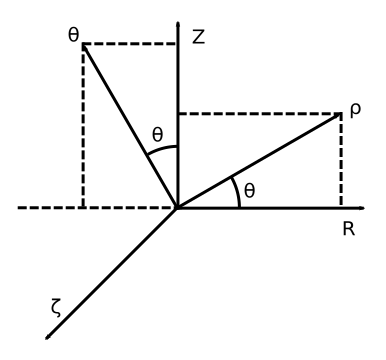
\includegraphics[width = 0.5 \textwidth]{%
    Chapters/TurbulenceMeasurements/figs/coordinate_geometry.pdf}
  \caption[Measurement coordinate system]{%
    Measurement coordinate system.
    Here, $R$ is the major-radial direction,
    $z$ is the lab-frame vertical direction,
    $\zeta$ is the toroidal angle,
    $\theta$ is the poloidal angle, and
    $\rho$ is a flux-surface label
    corresponding to the square root
    of the normalized toroidal magnetic-field flux.
  }
\label{fig:TurbulenceMeasurements:coordinate_geometry}
\end{figure}

Now, assuming that $\ExB$ advection
is the predominant contribution
to the PCI-measured phase velocity,
the line-integrated PCI measurements can be moderately localized.
To see this, note that the PCI measurements are Doppler shifted by
$\Delta \omega = \vect{k} \cdot \vect{v}$,
where $\vect{v}$ is the lab-frame velocity of the plasma.
Because $\vect{k} \perp \Beq$ by
(\ref{eq:TurbulenceMeasurements:kpropto}),
$\vect{k} \cdot \vect{v} = \vect{k} \cdot \vperp$, where
$\vperp$ is the velocity
perpendicular to the equilibrium magnetic field.
Defining the plasma frame via the ideal-MHD relation
$\vect{E} + \vperp \cross \Beq = 0$,
the perpendicular velocity is simply the $\ExB$ velocity
i.e.\ $\vperp = \vExB$.
Now, the electrostatic potential $\varphi = \varphi(\rho)$
is a flux function such that
the corresponding electric field is
$\vect{E} = -\nabla \varphi = E_r(\rho, \theta) \rhohat$.
The resulting $\ExB$ velocity is
\begin{align}
  \vExB
  =
  \frac{\vect{E} \times \Beq}{B_0^2}
  % \notag \\
  =
  \frac{E_r(\rho, \theta)}{B_0^2}
  \left(%
    B_{\theta} \zetahat
    -
    B_{\zeta} \thetahat
  \right)
  \label{eq:TurbulenceMeasurements:vExB}
\end{align}
such that the Doppler shift
$\Delta \omega = \vect{k} \cdot \vExB$ becomes
\begin{equation}
  \Delta \omega
  =
  \frac{%
    (\vect{k} \cdot \khat) E_r(\rho, \theta) \sin\theta}{%
    {\left[ B_{\zeta}^2 + {(B_{\theta} \sin\theta)}^2 \right]}^{1/2}}.
  \label{eq:TurbulenceMeasurements:Doppler_shift_from_ExB}
\end{equation}
Thus, the plasma's $\ExB$ rotation
results in a PCI-measured phase velocity
\begin{align}
  \vpciE
  =
  \frac{\Delta \omega}{k}
  =
  \frac{%
    \sgn(\vect{k} \cdot \khat) E_r(\rho, \theta) \sin\theta}{%
    {\left[ B_{\zeta}^2 + {(B_{\theta} \sin\theta)}^2 \right]}^{1/2}},
  \label{eq:TurbulenceMeasurements:PCI_phase_velocity_from_ExB}
\end{align}
where the sign function $\sgn(x)$
returns the sign of argument $x$.
Here, the plasma-frame phase velocity $v_{\text{ph}}$
of the fluctuations have been neglected,
which is valid when $|v_{\text{ph}}| \ll |\vpciE|$.
Further, note that the polarity of $\sin\theta$
switches at the plasma midplane (where $\theta = 0$) such that
(\ref{eq:TurbulenceMeasurements:PCI_phase_velocity_from_ExB})
switches signs when passing from above the plasma midplane
to below the plasma midplane.
Figure~\ref{fig:TurbulenceMeasurements:doppler_shift}
compares $\vpciE$ from
(\ref{eq:TurbulenceMeasurements:PCI_phase_velocity_from_ExB})
to the measured phase velocity $\vpcimeas$
of the high-$k$ turbulence observed in the left panel of
Figure~\ref{fig:TurbulenceMeasurements:Skf_pci}.

\begin{figure}
  \centering
  \includegraphics[width = 0.9 \textwidth]{%
    Chapters/TurbulenceMeasurements/figs/doppler_shift.pdf}
  \caption[Doppler-shift localization of high-$k$ turbulence]{%
    A comparison of the $\ExB$-induced phase velocity $\vpciE$ from
    (\ref{eq:TurbulenceMeasurements:PCI_phase_velocity_from_ExB})
    to the measured phase velocity $\vpcimeas$
    of the high-$k$ turbulence observed in the left panel
    of Figure~\ref{fig:TurbulenceMeasurements:Skf_pci}.
    The near degeneracy of $\vpciE$ with $\rho$
    corresponds to propagation above and below the plasma midplane.
    As the spatially filtering ``mask''~\cite{dorris_phd, dorris_rsi09}
    was not used in this experiment,
    it is not possible to determine whether
    $\vpcimeas$ corresponds to propagation above or below the midplane, so
    both $\vpcimeas$ and $-\vpcimeas$ are plotted.
  }
\label{fig:TurbulenceMeasurements:doppler_shift}
\end{figure}

As a brief aside, it should be emphasized
that the radial electric field $E_r$
in (\ref{eq:TurbulenceMeasurements:PCI_phase_velocity_from_ExB})
is \emph{not} a flux function.
To see this, recall that
the corresponding electrostatic potential
\emph{is} a flux function,
i.e.\ $\varphi = \varphi(\rho) = \varphi(\psi)$,
where $\psi$ is the flux-surface label
corresponding to the poloidal magnetic-field flux per radian.
Now,
\begin{align}
  E_r(\rho, \theta)
  &=
  -\left( \frac{\partial\varphi}{\partial r} \right)
  \notag \\
  &=
  -\left( \frac{d\varphi}{d\psi} \right)
  \left( \frac{\partial\psi}{\partial r} \right)
  \notag \\
  &=
  -\left( \frac{d\varphi}{d\psi} \right)
  \left( R B_{\theta} \right),
\end{align}
where the last line follows from the definition
of $\psi$ as the poloidal magnetic-field flux per radian.
The derivative $d\varphi / d\psi$
is a flux function because $\varphi$ is a flux function, and
this implies that $E_r / (R B_{\theta})$ is also a flux function.
Thus, the radial electric field at any point
within the last closed flux surface can be computed
from the radial electric field
along the outboard midplane (where $\theta = 0$) as follows
\begin{equation}
  \left.
  \frac{E_r}{R B_{\theta}}
  \right|_{\rho, \theta}
  =
  \left.
  \frac{E_r}{R B_{\theta}}
  \right|_{\rho, \theta = 0}.
  \label{eq:TurbulenceMeasurements:radial_electric_field}
\end{equation}


\section{TGLF modeling}
\begin{figure}[h!]
  \centering
  \includegraphics[width = \textwidth]{%
    Chapters/TurbulenceMeasurements/figs/wavenumber_conversion.pdf}
  \caption[Profiles of $k_y \rho_s$ for $k_R = \SI{1.5}{\per\centi\meter}$]{%
    Profiles of $k_y \rho_s$ for $k_R = \SI{1.5}{\per\centi\meter}$.
  }
\label{fig:TurbulenceMeasurements:wavenumber_conversion}
\end{figure}

\begin{figure}[h!]
  \centering
  \includegraphics[width = \textwidth]{%
    Chapters/TurbulenceMeasurements/figs/linear_stability_rho070.pdf}
  \caption[TGLF-predicted linear growth rates]{%
    TGLF-predicted linear growth rates.
    Filled symbols indicate electron modes, while
    unfilled symbols indicate ion modes.
  }
\label{fig:TurbulenceMeasurements:linear_stability}
\end{figure}

\begin{figure}[h!]
  \centering
  \includegraphics[width = \textwidth]{%
    Chapters/TurbulenceMeasurements/figs/density_spectra_rho070.pdf}
  \caption[TGLF-predicted density-fluctuation spectra]{%
    TGLF-predicted density-fluctuation spectra
  }
\label{fig:TurbulenceMeasurements:density_spectra}
\end{figure}


\bibliographystyle{plainurl}
\bibliography{references}
